\documentclass[a4paper,12pt]{article}
\usepackage[english,ukrainian,russian]{babel}
\linespread{1}
\usepackage{ucs}
\usepackage[utf8]{inputenc}
\usepackage[T2A]{fontenc}
\usepackage[paper=portrait,pagesize]{typearea}
\usepackage{amsmath}
\usepackage{bigints}
\usepackage{amsfonts}
\usepackage{graphicx}
\usepackage{amssymb}
\usepackage{cancel}
\usepackage{gensymb}
\usepackage{multirow}
\usepackage{rotate} 
\usepackage{pdflscape}
\usepackage{bigstrut}
\usepackage[pageanchor]{hyperref}
\usepackage{chngpage}
\usepackage{fancybox,fancyhdr}
\newcommand\tab[1][1cm]{\hspace*{#1}}
\newcommand{\RomanNumeralCaps}[1]{\MakeUppercase{\romannumeral #1}}
\usepackage[left=20mm, top=20mm, right=15mm, bottom=15mm, nofoot]{geometry}

\usepackage{verbatim}
\usepackage{enumerate}
\usepackage{listings}
\usepackage{xcolor}

\usepackage{mathtools}
\usepackage{MnSymbol}

\definecolor{codegreen}{rgb}{0,0.6,0}
\definecolor{codegray}{rgb}{0.5,0.5,0.5}
\definecolor{codepurple}{rgb}{0.58,0,0.82}
\definecolor{backcolour}{rgb}{0.95,0.95,0.92}

\lstdefinestyle{mystyle}{
	backgroundcolor=\color{backcolour},   
	commentstyle=\color{codegreen},
	keywordstyle=\color{blue},
	numberstyle=\tiny\color{codegray},
	stringstyle=\color{red},
	basicstyle=\ttfamily\footnotesize,
	breakatwhitespace=false,         
	breaklines=true,                 
	captionpos=b,                    
	keepspaces=true,                 
	numbers=none,                    
	numbersep=5pt,                  
	showspaces=false,                
	showstringspaces=false,
	showtabs=false,                  
	tabsize=4,
	frame=shadowbox
}

\lstset{style=mystyle}

% Language "Assembler"
\lstdefinelanguage{assembler}{
    keywords={MOV, LDR, CMP, BEQ, BLT, SUB, B, ADD, STR. DCD, LSL},
    sensitive=true,
    comment=[l]{;},  % Коментарі починаються з ;
    morestring=[b]",  % Рядки в лапках
    morestring=[b]',  % Рядки в одинарних лапках
}
\lstset{
    language=assembler,          % Встановлюємо мову
    basicstyle=\ttfamily,        % Шрифт для коду
    keywordstyle=\color{blue},   % Стиль для ключових слів
    commentstyle=\color{green},  % Стиль для коментарів
    stringstyle=\color{red},     % Стиль для рядків
    numbers=left,                % Номери рядків зліва
    numberstyle=\tiny,           % Стиль номерів рядків
    stepnumber=0,                % Номери для кожного рядка
    numbersep=5pt,               % Відстань до номера рядка
    frame=single,                % Рамка навколо коду
}

\begin{document}
    \pagestyle{fancy}
    \fancyhead{}
    \fancyhead[R]{ФІ-12 Завалій Олександр}
    \begin{center}
        \large{\textbf{Міністерство освіти і науки України\\
                Національний технічний університет України\\
                «Київський політехнічний інститут імені Ігоря Сікорського»\\
                Навчально-науковий Фізико-технічний інститут}}\\
        \hfill \break \hfill \break \hfill\break \hfill \break \hfill \break \hfill \break \hfill \break
        \hfill \break \hfill \break \hfill \break
        \begin{center}
            \normalsize{\textbf{Архітектура комп'ютерних систем\\
            Комп’ютерний практикум\\
            Робота №4}}
        \end{center}
    \end{center}
    \hfill \break \hfill \break \hfill \break \hfill \break \hfill \break \hfill \break \hfill \break
    \hfill \break \hfill \break \hfill \break \hfill \break 
    \begin{flushright}
        \large{ \hspace{35pt} Виконав:\\
            студент групи ФI-12\\
            Завалій Олександр\\} 
        \large{ \hspace{35pt} Перевірив:\\
        Козленко О.В.} 
    \end{flushright}
    \hfill \break \hfill \break \hfill \break \hfill \break \hfill \break \hfill \break \hfill \break
    \hfill \break
    \begin{center} \textbf{Київ-2024} \end{center}
    \thispagestyle{empty}

\newpage
    \begin{center}
        \section*{\bfseries{Робота №4.\\
        Основи побудови програми на асемблері в архітектурі x64 в операційній
        системі Windows з використанням WinAPI
    }}
    \end{center}
    \textbf{Мета:} \\
    \hangindent=1.5cm 
    \hangafter=+1 \noindent
    Ознайомитися з створенням базової програми мовою асемблер для
    операційної системи Windows 10 (або пізніше) архітектури х64 з використанням
    NASM. \\
    \begin{center}
        \Large{Варіант №4}
    \end{center}
    Зміст індивідуального завдання:
    \begin{itemize}
        \item Визначити дані: \\
        $a(1) \rightarrow 12,\: 
        a(2) \rightarrow 6,\: 
        a(3) \rightarrow 17,\: 
        c1 \rightarrow 23,\: 
        c2 \rightarrow 16$
        \item Занести в регістри такі величини: \\
        $RAX \rightarrow a(1) + a(3) - a(2),\:
        RBX \rightarrow \dfrac{a(1)}{a(2)},\:
        RCX \rightarrow c1+c2,\:
        RDX \rightarrow a\stackrel{rc\rightarrow 4}{1}$
        \item Організувати цикл, послідовно зменшуючи число у регістрі RСХ на 5. У
        циклі збільшувати число, що знаходиться у регістрі RВХ на величину, що
        знаходиться у регістрі RАХ, та зменшувати на величину, що знаходиться у
        регістрі RСХ, поки значення RСХ не стане менше 5.
        \item Створити MessageBox та записати у нього відповідні значення регістру RCX після всіх
        операцій.
    \end{itemize}

\newpage
    \begin{center}
        \Large{Code}
    \end{center}
    \begin{lstlisting}[language=assembler]
global start
NULL equ 0
MB_OK equ 0
     extern MessageBoxA
     extern ExitProcess

section .data
    a1 equ 12
    a2 equ 6
    a3 equ 17
    c1 equ 23
    c2 equ 16
    text: db 'rcx: ',0
    title: db 'Result',0

section .bss
    numbuf resb 20

section .text

itoa:
    push rbp
    mov rbp,rsp
    sub rsp,8
    mov rax,rcx
    lea rdi,[numbuf+10]
    mov rcx,10
    mov qword [rbp-8],0

.divloop:
    xor rdx,rdx
    idiv rcx
    add rdx,0x30
    dec rdi
    mov byte [rdi],dl
    inc qword [rbp-8]
    cmp rax,0
    jnz .divloop
    mov rax,rdi
    leave
    ret
    \end{lstlisting}

\newpage
    \begin{lstlisting}[language=assembler]
start:
     mov rax, a1
     add rax, a3
     sub rax, a2
     push rax
     mov rdx, 0
     mov rax, a1
     mov rbx, a2
     div rbx
     mov rbx, rax
     pop rax
     mov rcx, c1
     add rcx, c2
     mov rdx, a1
     rcr rdx, 4
loop:
     cmp rcx, 5
     jl loopend
     sub rcx, 5
     add rbx, rax
     sub rbx, rcx
     jmp loop

loopend:
     call itoa
     mov rcx, rbx
     mov rbx, [rax]
     mov [text+5], rbx
     sub rsp, 40
     mov r9, MB_OK
     mov r8, title
     mov rdx, text
     mov rcx, NULL
     call MessageBoxA

quit:
     xor rcx, rcx
     call ExitProcess
    \end{lstlisting}

\newpage
    \begin{figure}[h!]
        \begin{minipage}[h]{1\linewidth}
            \centering
            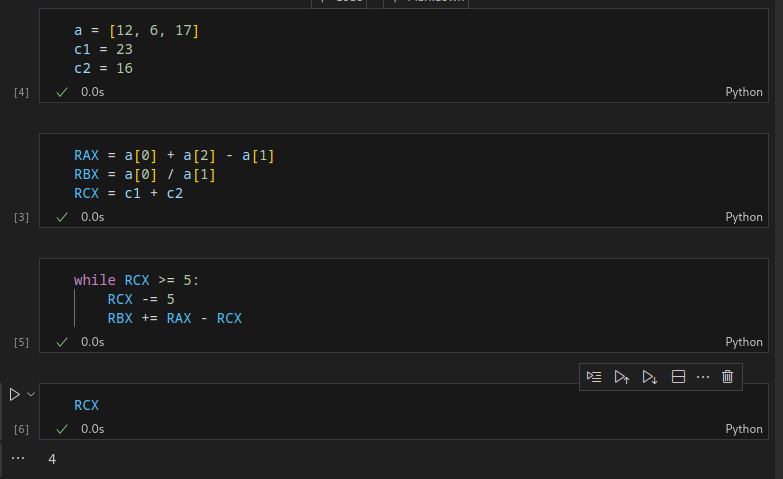
\includegraphics[width=1\linewidth]{Prt sc/Python_code.png}  
        \end{minipage}
    \end{figure}

    \begin{center}
        \Large{Results}
    \end{center}
    \begin{figure}[h!]
        \begin{minipage}[h]{1\linewidth}
            \centering
            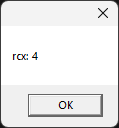
\includegraphics[width=0.2\linewidth]{Prt sc/Result.png}  
        \end{minipage}
    \end{figure}
    Результати роботи програм співпадають.




\end{document}